% !TeX root = main.tex
% =====================================================================
% Supporting appendices for
%   "Composition Without Grammar: Next-Token Models Miss Regulatory
%    Structure in Bacterial DNA"  --  ICBINB-BIO @ NeurIPS 2026
% ---------------------------------------------------------------------
% SUBMISSION: this file is \input by main.tex after Appendix B, so its sections
% continue the appendix lettering in the same PDF. Compiling supplementary.tex
% alone is only for local inspection; do not submit a separate appendix PDF.
% =====================================================================
\ifdefined\ICBINBSupplementInMain
  \clearpage
  \FloatBarrier
\else
\documentclass{article}

\PassOptionsToPackage{numbers,sort&compress}{natbib}
\usepackage[dblblindworkshop]{neurips_2026}
\workshoptitle{I Can't Believe It's Not Better (ICBINB): Failure Modes of AI in Biology}

\usepackage[utf8]{inputenc}
\usepackage[T1]{fontenc}
\usepackage{hyperref}
\hypersetup{hidelinks}
\usepackage{url}
\usepackage{booktabs}
\usepackage{amsmath,amssymb,amsfonts}
\usepackage{nicefrac}
\usepackage{microtype}
\usepackage{xcolor}
\usepackage{graphicx}
\usepackage{placeins}

% Float placement: identical to main.tex, so the standalone build lays the
% figures out the way they appear in the submission PDF.
\renewcommand{\topfraction}{0.95}
\renewcommand{\bottomfraction}{0.7}
\renewcommand{\textfraction}{0.05}
\renewcommand{\floatpagefraction}{0.90}
\setcounter{topnumber}{2}
\setcounter{totalnumber}{4}

\renewcommand{\thesection}{\Alph{section}}
\numberwithin{figure}{section}
\numberwithin{table}{section}
\numberwithin{equation}{section}

\title{Supporting Appendix\\[0.4em]
\large Composition Without Grammar: Next-Token Models Miss Regulatory
Structure in Bacterial DNA}

\author{Marc Augustine Sojerido Amil \and Aleksej Zelezniak}

\begin{document}
\maketitle

This document collects supporting analyses for the main paper. In the submitted
PDF these sections continue after Appendix B rather than appearing as a separate
file.
\fi

% Camera-ready revision marking. Defined here with \providecommand so that this
% file also compiles standalone; main.tex defines the same macro.
\providecommand{\rev}[1]{\begingroup\color{red}#1\endgroup}

% =====================================================================
\section{The gene--upstream association of Fig.~1A}
\label{app:fig1a}

\paragraph{Pairs and controls.} We paired $727$ \emph{E.~coli} K-12 singletons
with singleton orthologues from MMseqs2 Gammaproteobacterial families, requiring
$\ge30\%$ BLASTP identity, $\ge70\%$ coverage and a full $200$\,bp upstream. This
gave $22{,}393$ pairs from $408$ genomes. Controls were unrelated singletons from
the same target genome, length-matched to $\pm10\%$, thereby matching genome
composition and phylogenetic distance while removing homology.

\rev{\paragraph{Why conserved gene order does not drive this panel.} Both filters
above are applied to every gene on both sides of every pair, and together they
rule out the obvious synteny confound. ``Singleton'' means an operon size of one,
so the gene is not co-transcribed with a neighbour; ``a full $200$\,bp upstream''
means the annotated distance to the nearest upstream feature is at least
$200$\,bp, so the window stops before the neighbouring gene and contains no
neighbouring coding sequence. A window here is therefore intergenic by
construction, and conserved gene order cannot produce upstream similarity by
placing a conserved CDS inside it. The controls inherit the same two filters, so
test and control pairs are matched on gene architecture as well as on genome
composition, phylogenetic distance and upstream length. The coverage figures
quoted in Appendix~\ref{app:cds-composition} ($41\%$ and $32\%$ of windows clear
of the nearest upstream feature) describe the CDS-prompted benchmark, which
applies no such distance requirement, and do not apply to this panel.

One weaker version of the concern does survive. Clearing the neighbouring
\emph{gene} does not clear shared regulatory architecture: where a gene and its
orthologue both lie downstream of a divergently transcribed neighbour, the
conserved sequence in the window may be that neighbour's promoter rather than the
focal gene's. This remains regulatory sequence, but it is not necessarily
evidence of coevolution with the focal CDS.}

\paragraph{Upstream similarity ($D_2^*$).} A direct $4$-mer comparison can be
misleading because two AT-rich sequences share many short words even when they
are unrelated. We therefore compare observed counts with those expected from
each sequence's own background composition. For a $4$-mer $w$, $X_w$ is its
observed count and $\mathbb{E}[X_w]$ its expected count. The expectation uses an
order-$2$ Markov model, which predicts each base from the previous two bases:
$\mathbb{E}[X_w]=N(w_{1:3})N(w_{2:4})/N(w_{2:3})$, where $N(u)$ counts substring
$u$ and the subscripts select the first three, last three and middle two bases of
$w$. We then calculate
%
\begin{equation}
\tilde{X}_w = \frac{X_w - \mathbb{E}[X_w]}{\sqrt{\mathbb{E}[X_w]}},
\qquad
D_2^{*} = \frac{\sum_w \tilde{X}_w \tilde{Y}_w}
               {\sqrt{\sum_w \tilde{X}_w^{2}}\;\sqrt{\sum_w \tilde{Y}_w^{2}}},
\end{equation}
%
Here, $\tilde X_w$ is positive when $w$ occurs more often than expected and
negative when it occurs less often; $\tilde Y_w$ is the same value for the second
sequence. $D_2^*$ compares these corrected patterns across all $256$ $4$-mers:
$1$ means the patterns match and $0$ means no agreement. It therefore measures
similarity beyond that explained by background base composition.

\paragraph{Third-position identity.} A codon contains three bases, and changes at
its third base often do not change the encoded amino acid. For each aligned gene
pair, we therefore calculate the fraction of codons with the same third base,
using pairs with at least $30$ aligned codons. A high value indicates more closely
related coding sequences and a low value greater evolutionary divergence. This is
the $x$ axis in Fig.~1A and measures relatedness, not gene function.

% =====================================================================
\section{The upstream-only benchmark}
\label{app:benchmark-composition}

Not all five sigma factors build promoters from $-35$/$-10$ elements
($\sigma^{54}$ uses $-24$/$-12$), so we write \emph{distal} and \emph{proximal}
box throughout. Figure~\ref{fig:benchmark-composition} summarizes the dataset and
controls, Fig.~\ref{fig:sigma-logos} shows the box motifs, and
Fig.~\ref{fig:spacerhist} shows the spacer-length distributions.

\begin{figure}[htbp]
  \centering
  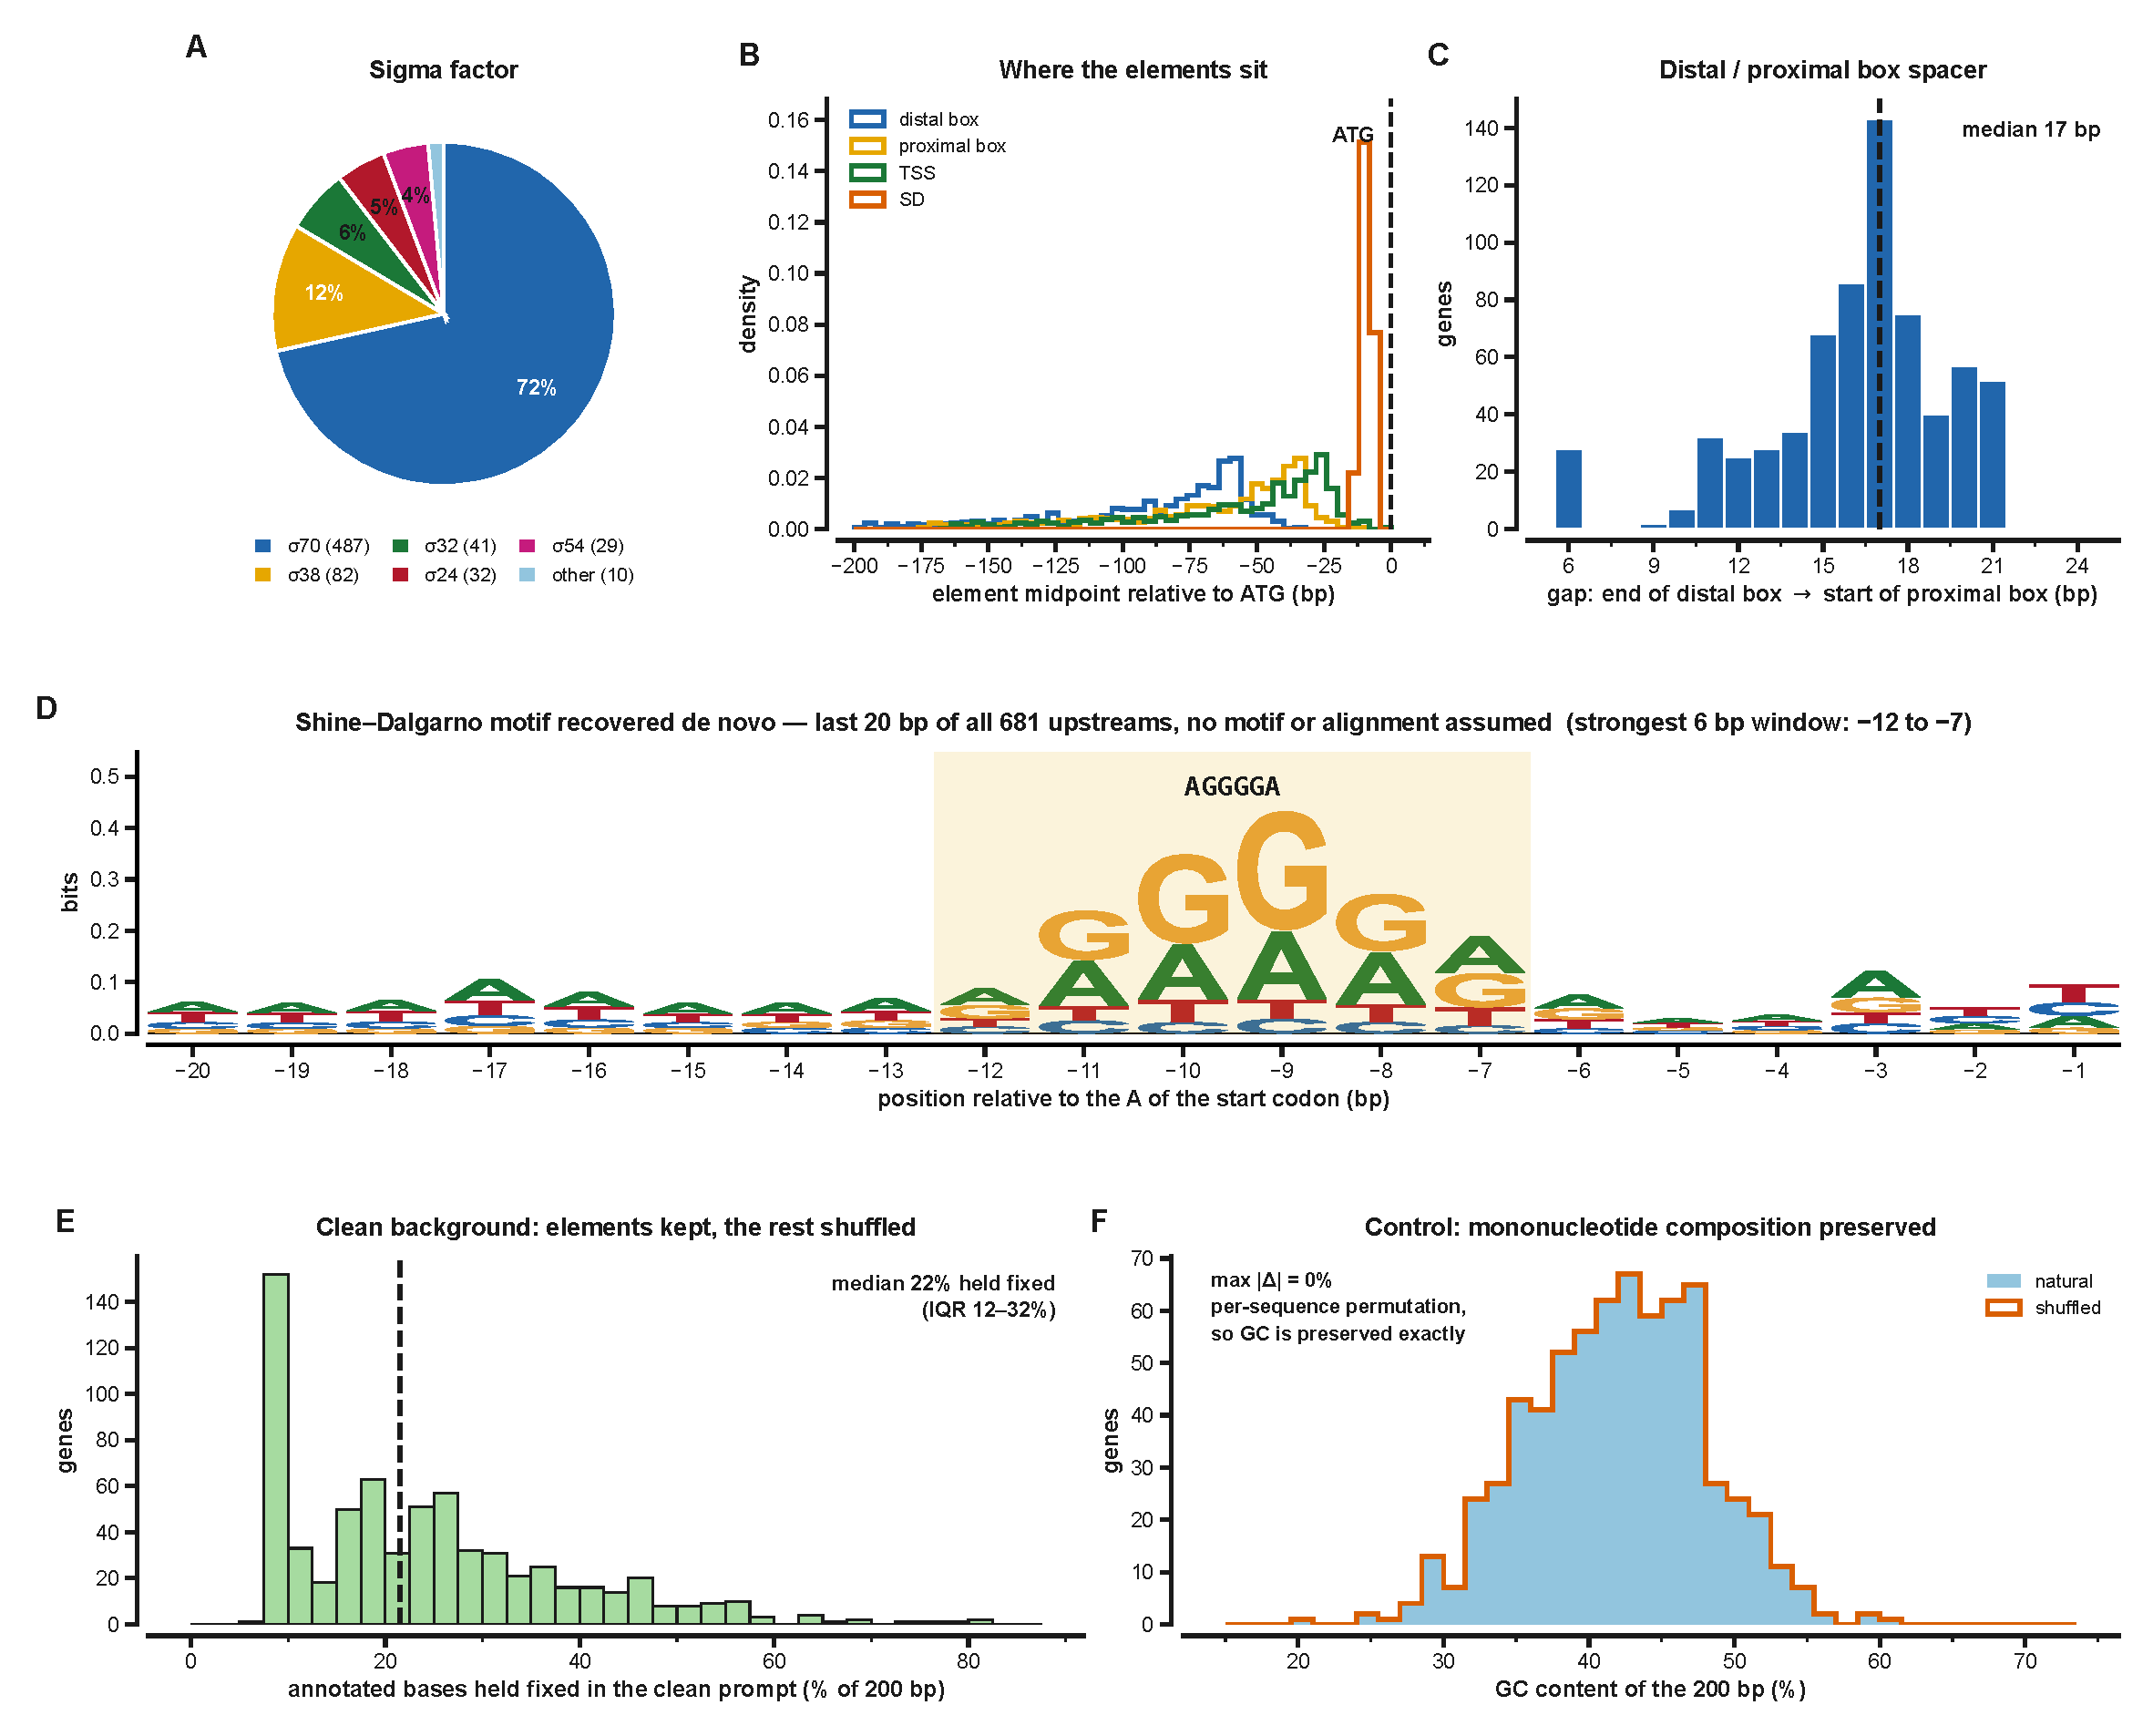
\includegraphics[width=0.95\linewidth]{figures/upstream_only_dataset_supp.pdf}
  \caption{\textbf{Composition and controls of the upstream-only benchmark.}
  $681$ RegulonDB-annotated \emph{E.~coli} genes with up to $200$\,bp before the
  start codon. \textbf{(A)} Sigma-factor counts; promoter-box analyses use the 671
  genes in the five displayed factors, while one $\sigma^{28}$ and nine unassigned
  genes remain in Shine--Dalgarno analyses. \textbf{(B)} Annotated element
  midpoints relative to the start codon. \textbf{(C)} Distal-to-proximal box
  spacing. \textbf{(D)} Information logo for the final $20$\,bp.
  \textbf{(E)} Fraction of each clean prompt held fixed as an annotated element.
  \textbf{(F)} Natural and clean-prompt GC content. The Shine--Dalgarno emerges de
  novo in (D) with no motif assumed, and the clean background holds every annotated
  element at its real position (E) while preserving mononucleotide composition
  exactly (F), so a score against it cannot be explained by composition.}
  \label{fig:benchmark-composition}
\end{figure}

\begin{figure}[htbp]
  \centering
  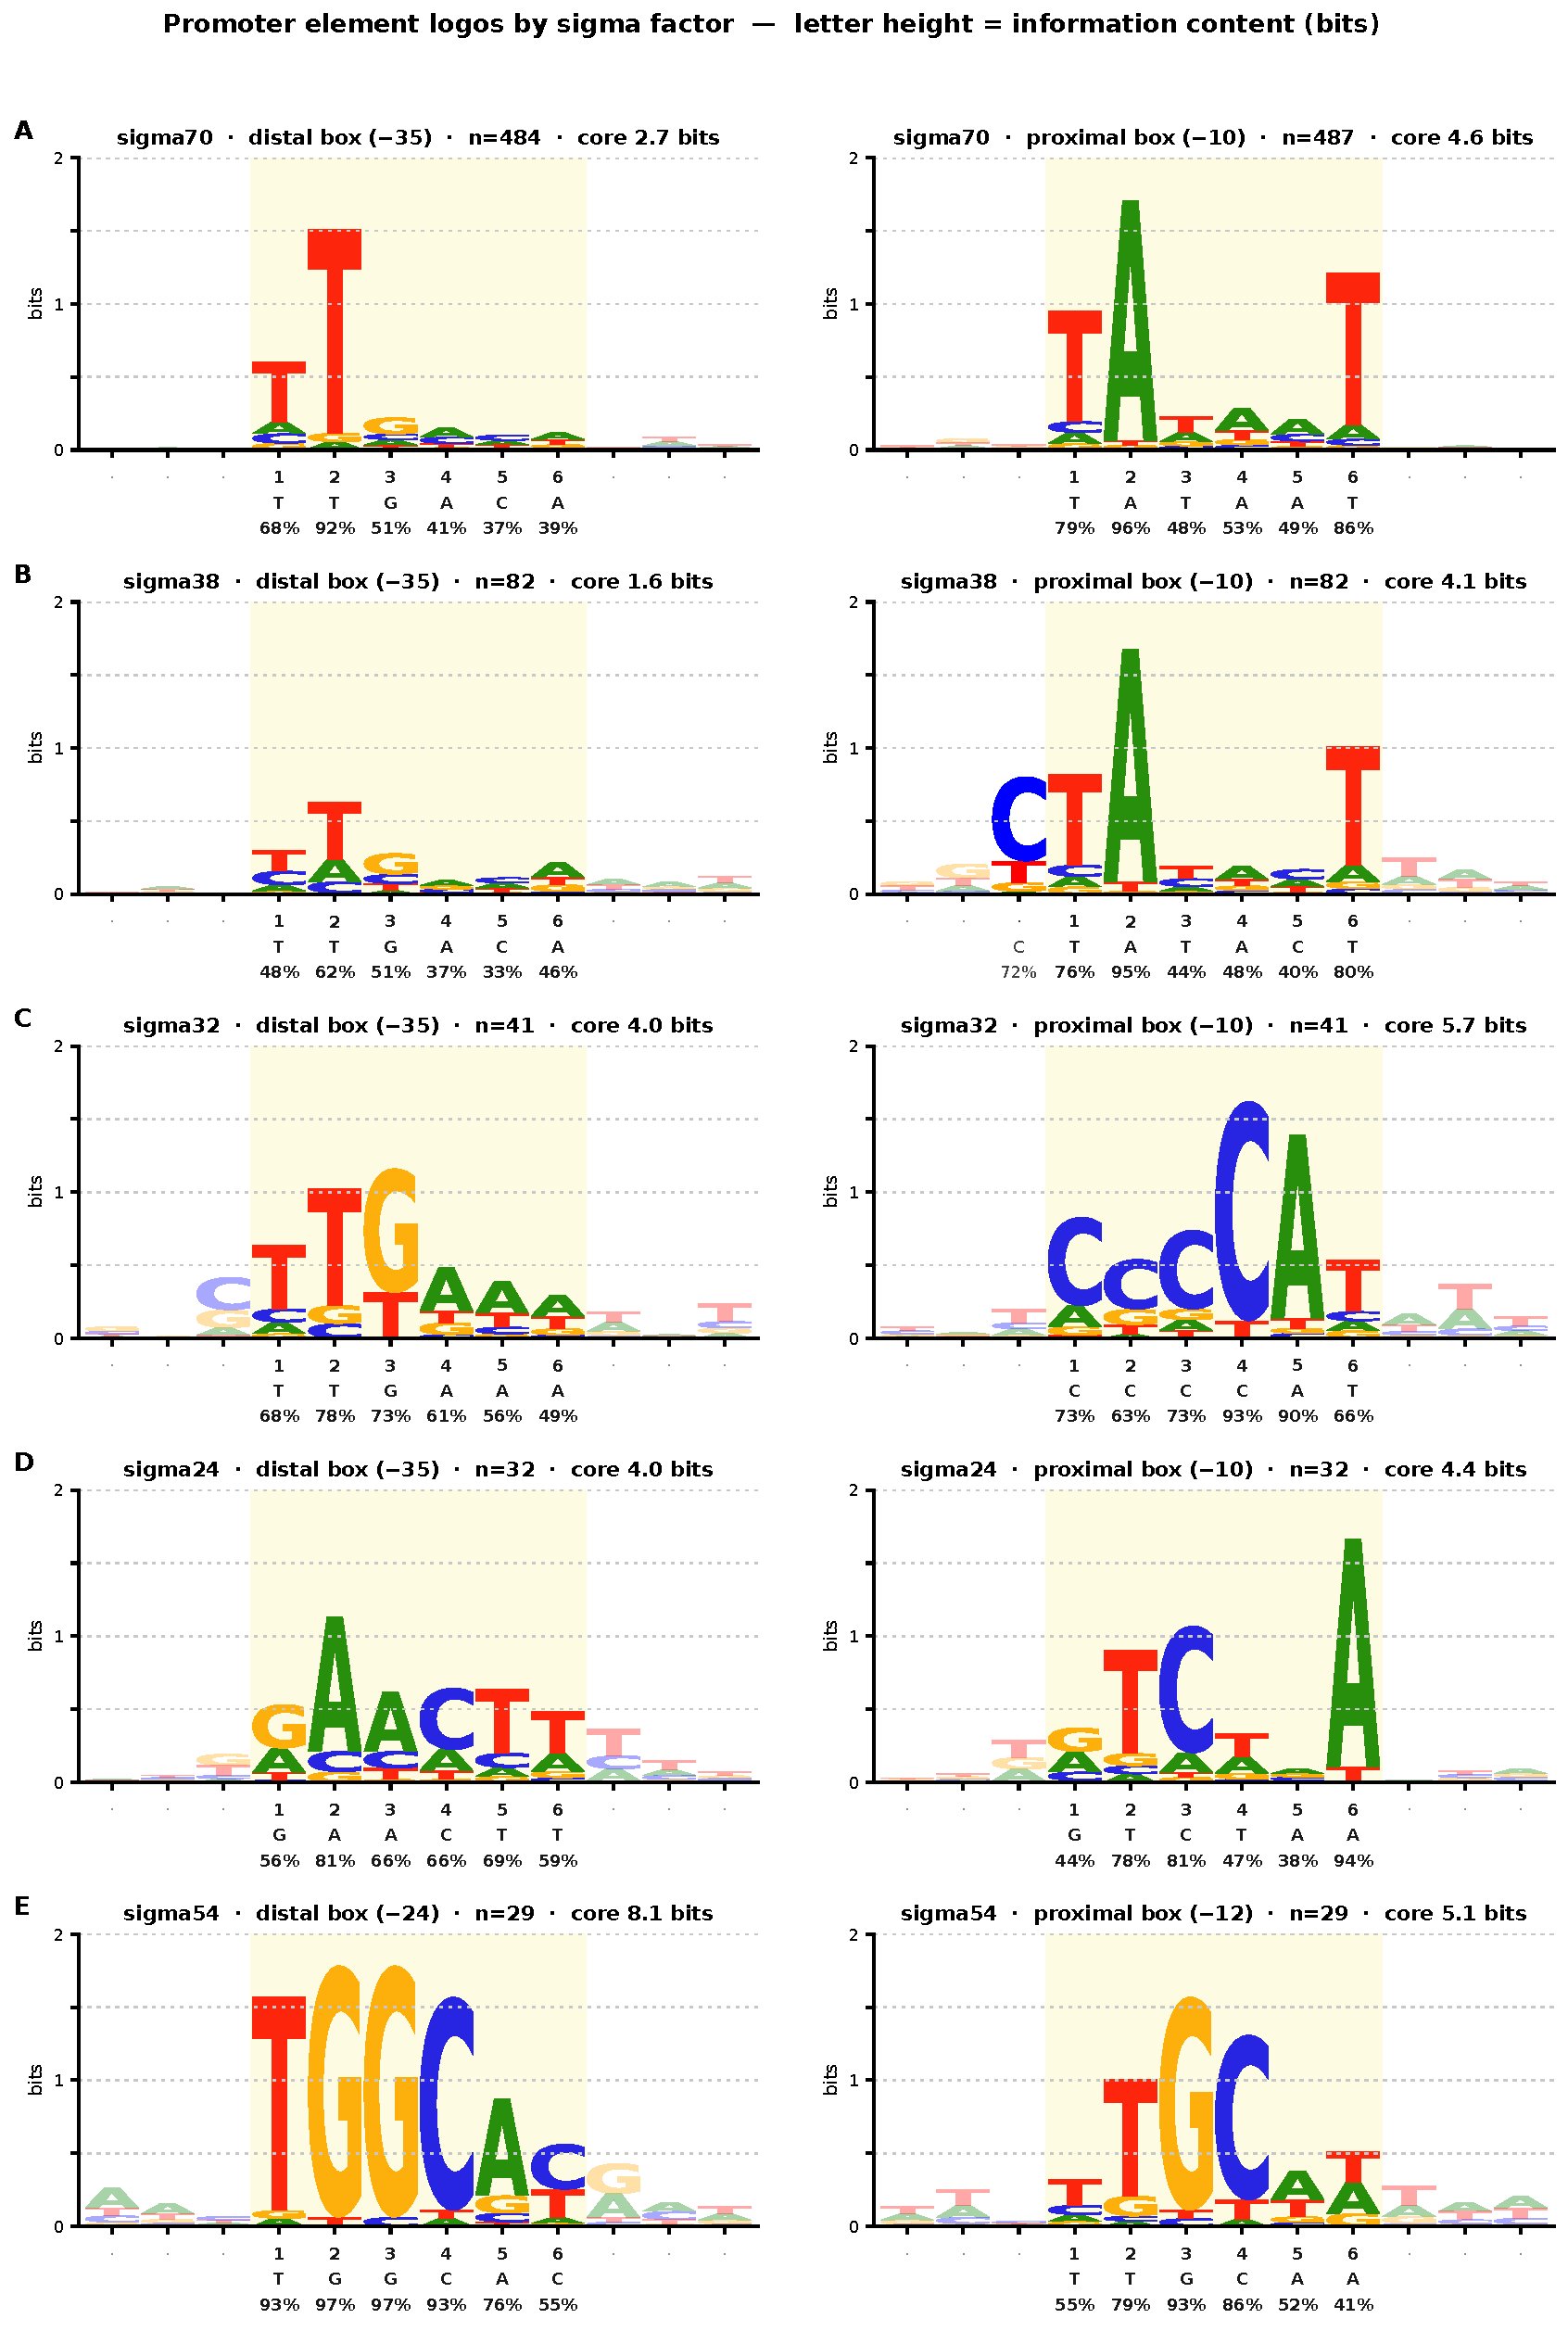
\includegraphics[width=0.88\linewidth]{figures/upstream_only_logos.pdf}
  \caption{\textbf{Promoter-box logos by sigma factor.}
  Information logos for distal and proximal boxes in RegulonDB-annotated
  \emph{E.~coli} upstreams ($n\ge 25$ per factor). Six-base cores are shaded and
  three-base flanks are faded; the modal base and frequency are printed below each
  core position. Windows are anchored at the distal box's $5'$ end and the
  proximal box's $3'$ end; the benchmark reproduces the published consensus for
  every factor.}
  \label{fig:sigma-logos}
\end{figure}

% =====================================================================
\begin{figure}[htbp]
  \centering
  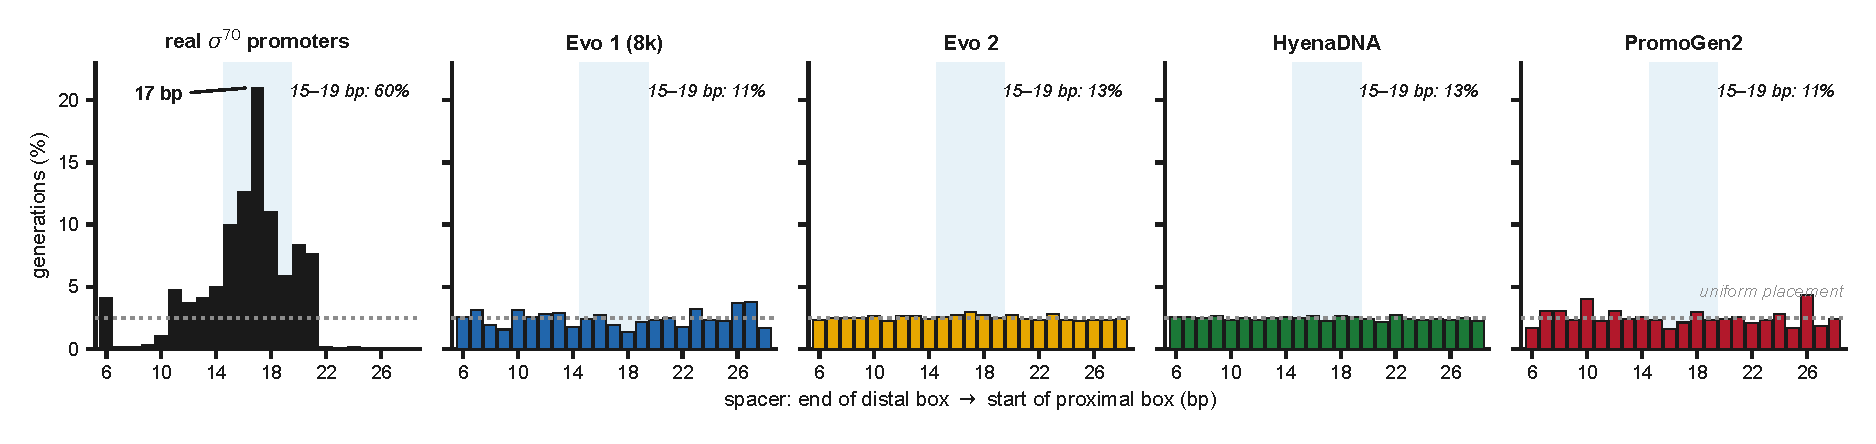
\includegraphics[width=\linewidth]{figures/supp_spacer_histograms.pdf}
  \caption{\textbf{The spacer distribution, one histogram per model.} Each model's
  best-scoring proximal-box position, read as a spacer from the distal box, on a
  shared $y$-axis. Real $\sigma^{70}$ promoters concentrate at $17$\,bp; every model
  spreads the spacer almost uniformly. Shading marks the canonical $15$--$19$\,bp
  window, the dotted line uniform placement ($2.5\%$ per offset), and the inset
  number the fraction inside the canonical window. Real promoters fall in the
  canonical window $60.5\%$ of the time and at exactly $17$\,bp $21.0\%$ of the
  time; the models give $10.7$--$13.5\%$ and $2.0$--$3.0\%$, against $12.5\%$ and
  $2.5\%$ for uniform placement. Presence is not the failing quantity: the scan
  finds a box in $93$--$97\%$ of generations and in $95$--$97\%$ of shuffles of
  those same generations, because an AT-rich stretch supplies a proximal-box-like
  hexamer by chance.}
  \label{fig:spacerhist}
\end{figure}


% =====================================================================
\FloatBarrier
\section{What the models were trained on}
\label{app:traincomp}

Non-coding bases---those outside predicted coding regions---are an upper bound on
what a model could have learned promoters from.

\begin{figure}[!htbp]
  \centering
  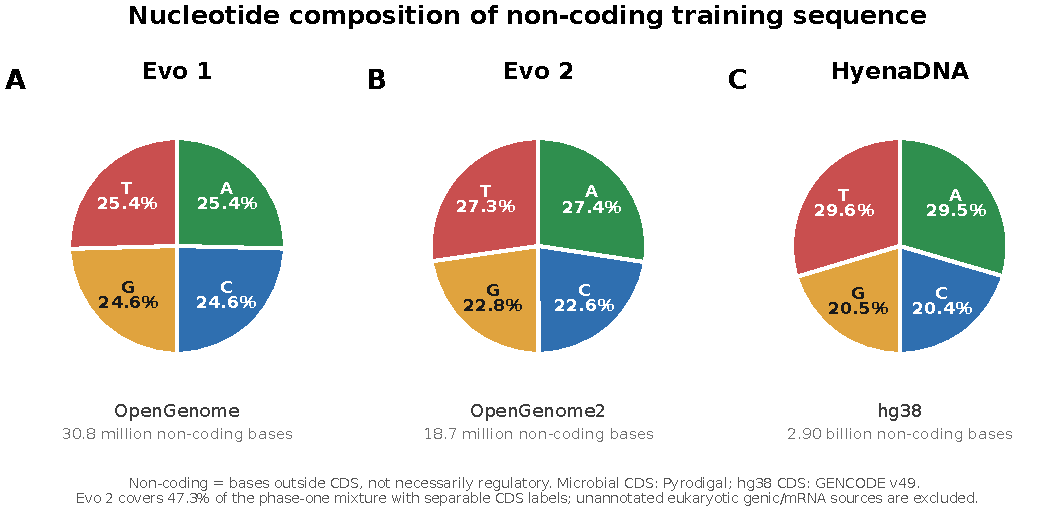
\includegraphics[width=\linewidth]{figures/supp_training_composition.pdf}
  \caption{\textbf{Nucleotide composition of the non-coding sequence in each
  model's training corpus.} Bases outside predicted CDS intervals, sampled
  reproducibly from each released corpus. \textbf{(A)}~Evo\,1 (OpenGenome).
  \textbf{(B)}~Evo\,2 (OpenGenome2), restricted to the $47.3\%$ of the phase-one
  mixture whose records carry separable CDS labels; unannotated eukaryotic
  genic and mRNA sources are excluded. \textbf{(C)}~HyenaDNA (hg38). PromoGen2 is
  omitted: it is trained on curated promoter sequence, not whole genomes. The
  corpora differ ($50.8\%$, $54.7\%$ and $59.2\%$ AT) but the outputs do not
  ($60.4\%$, $57.7\%$ and $59.7\%$, against $61.5\%$ in real \emph{E.~coli}
  upstreams), so matching the composition of a bacterial upstream is a low bar.}
  \label{fig:traincomp}
\end{figure}

% =====================================================================
\FloatBarrier
\section{Composition of the CDS-prompted benchmark}
\label{app:cds-composition}

The benchmark contains protein-coding, in-frame singletons of at least $30$
codons with a complete $200$\,bp upstream: $1{,}885$ from \emph{E.~coli} and
$1{,}272$ from \emph{B.~subtilis}. Only $41\%$ and $32\%$ of these windows are
clear of the nearest upstream feature, so overlap is a stratifier; restricting
the analysis to singletons limits inference to independently regulated genes.
\rev{This coverage figure applies to the CDS-prompted benchmark only. The Fig.~1A
pairs additionally require at least $200$\,bp to the nearest upstream feature
(Appendix~\ref{app:fig1a}), so every window in that panel is clear.}

The seven conditions are defined in Table~\ref{tab:conditions}. C1 and C2
rearrange codons, C3 substitutes another gene and C4 removes the CDS. C5 shuffles
the first $30$ codons and C6 the remainder, contrasting the region nearest the
ribosome-binding site with the region nearest the generation point. Cross-gene
upstream identity is near the composition floor ($0.255$ and $0.269$), so a
species-generic upstream is not a gene-specific match.

\begin{table}[htbp]
  \centering
  \footnotesize
  \caption{\textbf{The seven CDS perturbation conditions.} Percentages are mean
  nucleotide changes in \emph{E.~coli}/\emph{B.~subtilis}. The start codon is
  fixed; shuffled conditions preserve length, codon counts and GC, while C3 is
  length-matched and GC-matched in the mean. KL results are in
  Table~\ref{tab:kl}; C2 is shown in Fig.~\ref{fig:cds}C.}
  \label{tab:conditions}
  \begin{tabular}{@{}llcc@{}}
    \toprule
    & CDS given to the model & nt changed (E/B) & CDS GC vs.\ C0 \\
    \midrule
    C0 & the real CDS (reference)                      & ---            & --- \\
    C1 & synonymous codons permuted, protein unchanged & $20.0/20.6\%$  & identical \\
    C2 & codon order shuffled                          & $72.0/71.2\%$  & identical \\
    C3 & a different, length-matched gene's CDS        & $71.9/71.9\%$  & matched in the mean \\
    C4 & removed entirely                              & ---            & --- \\
    C5 & codons 1--30 shuffled; remainder fixed        & $10.7/11.9\%$  & identical \\
    C6 & codons 31--end shuffled; first 30 fixed       & $60.8/58.7\%$  & identical \\
    \bottomrule
  \end{tabular}
\end{table}

\ifdefined\ICBINBSupplementInMain
  \FloatBarrier
\else
  \bibliographystyle{plainnat}
  \bibliography{Literature_Sources/references}
  \end{document}
\fi
